\subsection{Recap: Software Product Lines and Features}
\begin{frame}{\myframetitle\ \mytitlesource{\fospl} \todo{SPL Def citation}}
	\begin{mycolumns}
		\mydefinition{Software Product Line}{
			\begin{itemize}
				\item set of software-intensive systems (aka products)
				\item sharing a common, managed set of \emph{features}
				\item satisfying the needs of a domain
				\item developed from a common set of core assets (reuse)
			\end{itemize}
		}
		\mydefinition{Feature}{
			\begin{itemize}
				\item domain abstraction
				\item used for communication by stakeholders (e.g., manager, developer, tester, customer, marketing)
				\item specifies differences between products
			\end{itemize}
		}
	\mynextcolumn
		\myexample{Examples}{
			\begin{itemize}
				\item \todots
			\end{itemize}
		}
		\todo{scoping?}
	\end{mycolumns}
\end{frame}

\subsection{Configuring Features}
% \begin{frame}{\myframetitle}
% 	\todo{examples for simple feature models without (or with few) dependencies}
	
% 	\todo{Configuring a Sandwich}

% 	\todo{Configuring ...}
% \end{frame}

% \xkcd{2369}

\subsection{Configuring Features with Dependencies}

\begin{frame}{\myframetitle}
	\begin{mycolumns}[columns=3,widths={40,20,40}]
		\myexampletight{Ordering a Waffle \ldots}{
			\pic[width=\textwidth]{waffle-feature-model}
		}
		\mynextcolumn
		\myexampletight{\ldots With Sugar}{
			\pic[width=\textwidth]{waffle-sugar}
		}
		\myexampletight{\ldots With Cherries}{
			\pic[width=\textwidth]{waffle-cherries}
		}
		\mynextcolumn
		\mynote{This is Nice, But \ldots}{
			\begin{itemize}
				\item plate and sugar seem to always be included, a fork is only included for some orders\\
					$\Rightarrow$ limitations seem arbitrary
				\item children get special treatment\\
					$\Rightarrow$ order process is unfair
				\item what exactly am I paying for?\\
					$\Rightarrow$ investments are unclear
				\end{itemize}
		}
		\mydefinition{In This Lecture}{
			\begin{enumerate}
				\item how to model and configure features and their dependencies?
				\item how to store and communicate?
				\item how to analyze and understand?
			\end{enumerate}
		}
	\end{mycolumns}
\end{frame}

% \begin{frame}{\myframetitle}
% 	\partofpage{70}{\myexampletight{Configuring a Notebook}{\only<1,3->{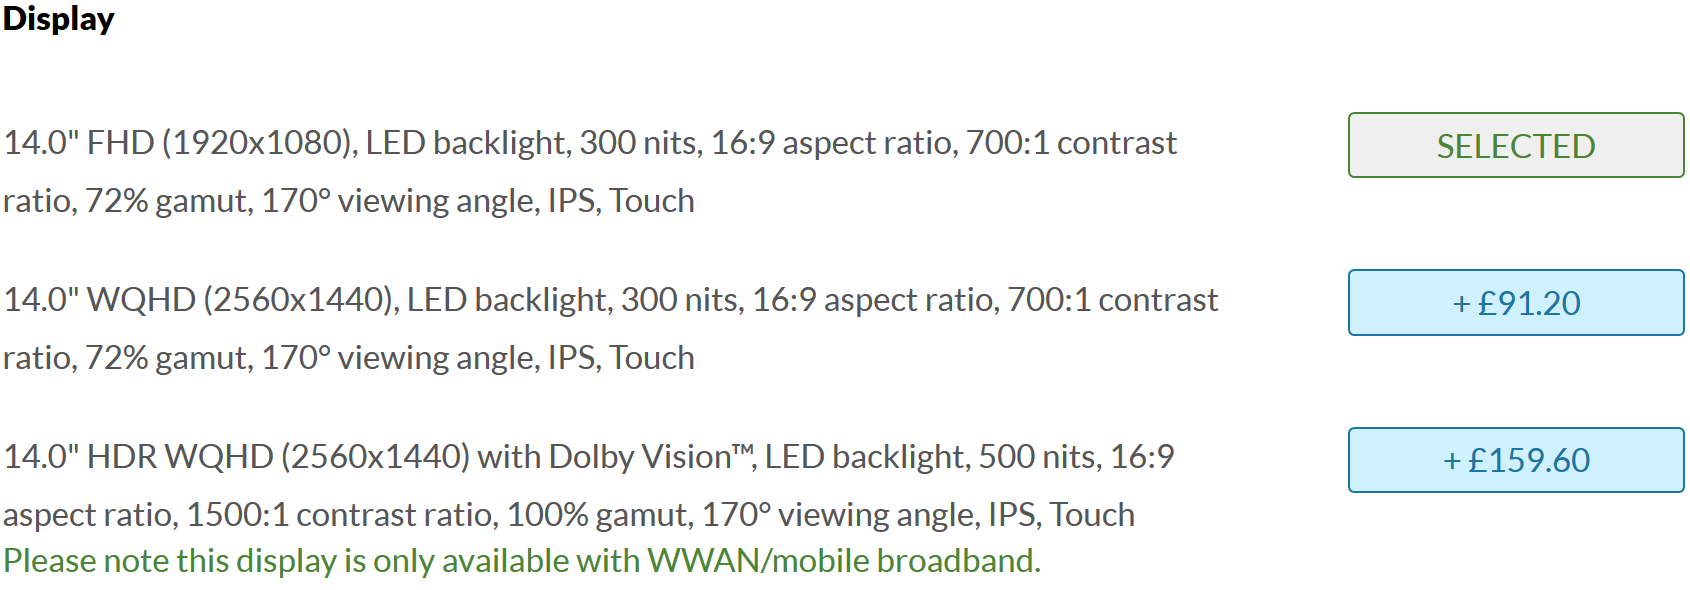
\includegraphics[width=\linewidth]{thinkpad-x1-yoga-display}}\only<2|handout:0>{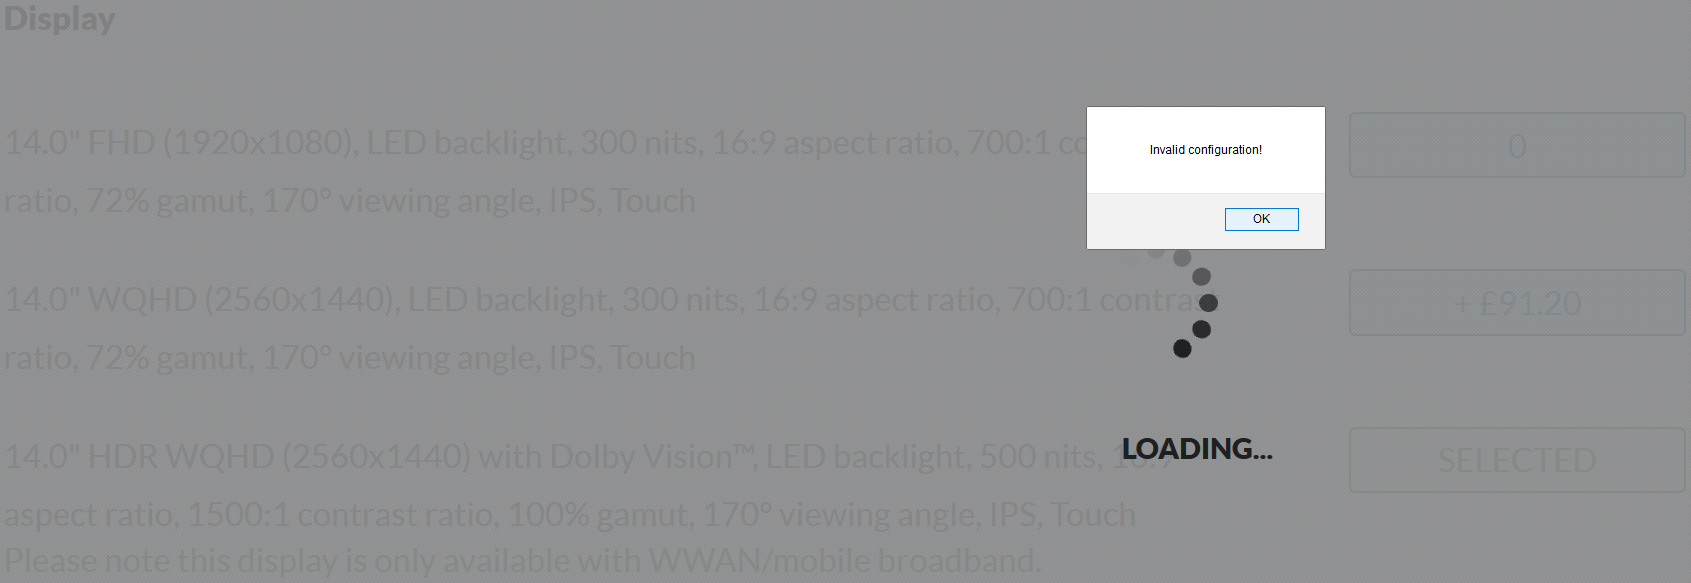
\includegraphics[width=\linewidth]{thinkpad-x1-yoga-display-invalidconf}}}}
% \end{frame}

% \begin{frame}{\myframetitle}
% 	\partofpage{70}{\myexampletight{Still Configuring a Notebook}{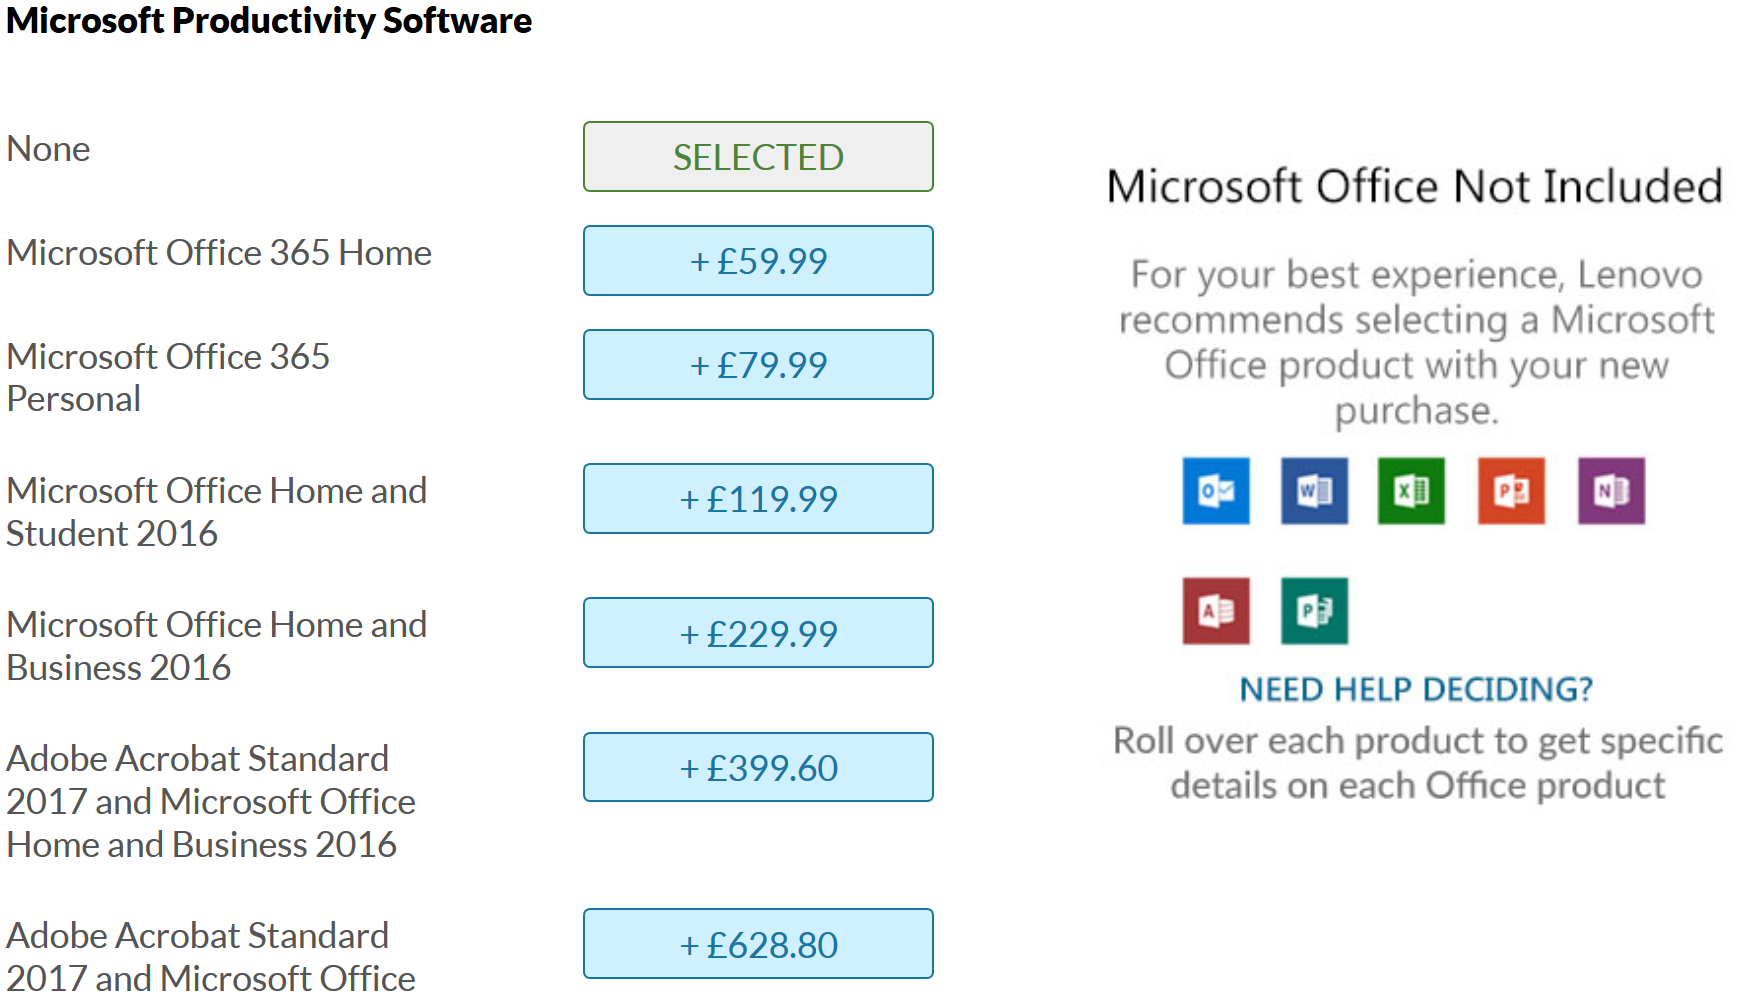
\includegraphics[width=\linewidth]{thinkpad-x1-yoga-office}}}
% \end{frame}

% \begin{frame}{\myframetitle}
% 	~\hfill\partofpage{60}{\myexampletight{Configuring a Car}{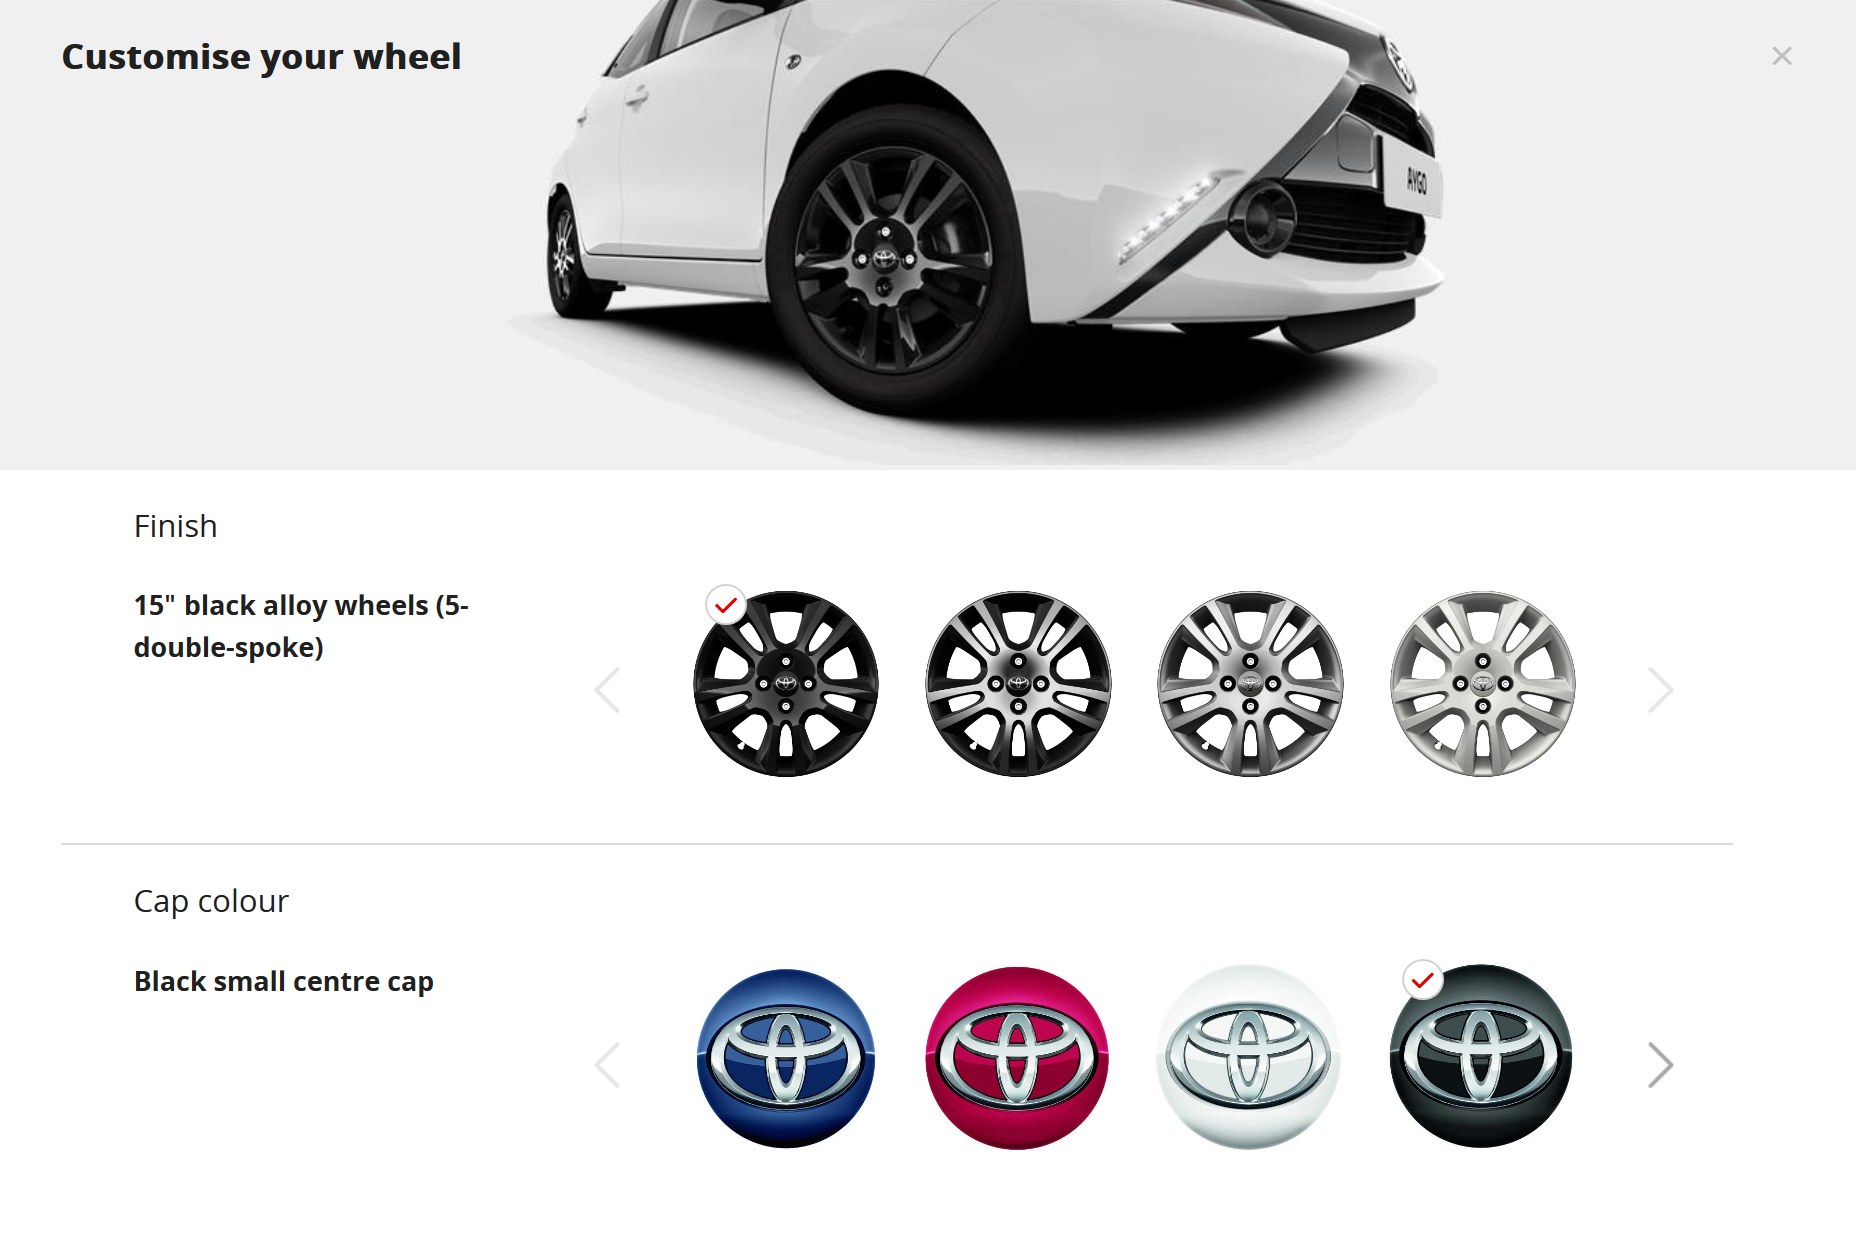
\includegraphics[width=\linewidth]{toyota-aygo-wheels}}}
% \end{frame}

% \begin{frame}{\myframetitle}
% 	~\hfill\partofpage{60}{\myexampletight{Configuring a Car with a Weird Price}{\centering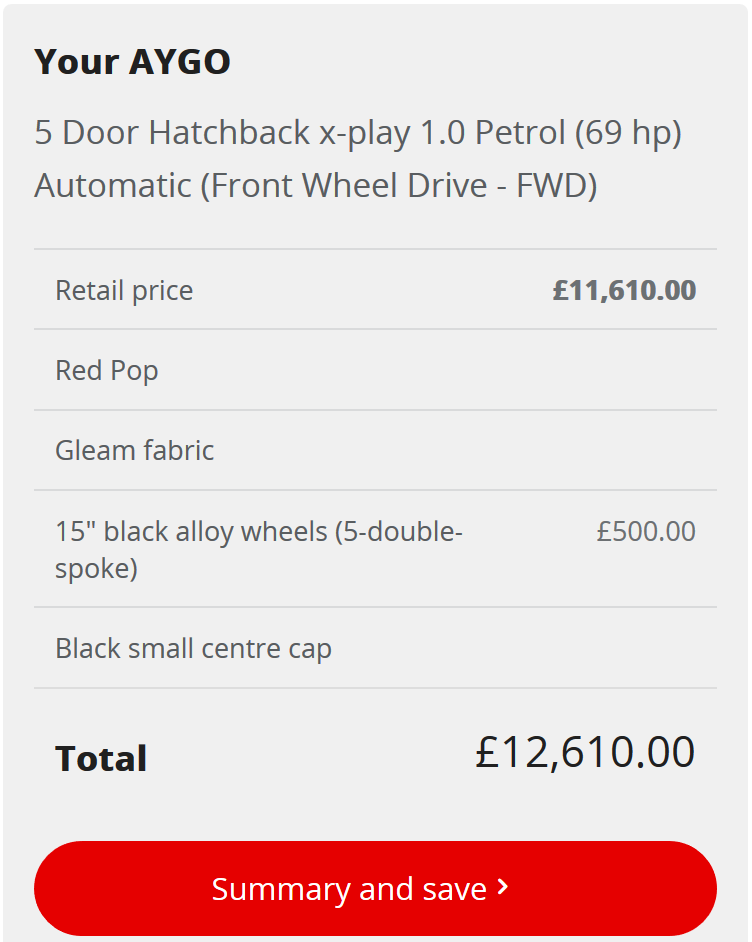
\includegraphics[width=.55\linewidth]{toyota-aygo-costs}}}
% \end{frame}

% \begin{frame}{\myframetitle}
% 	~\hfill\partofpage{60}{\myexampletight{Configuring a Car with 8 Wheels!}{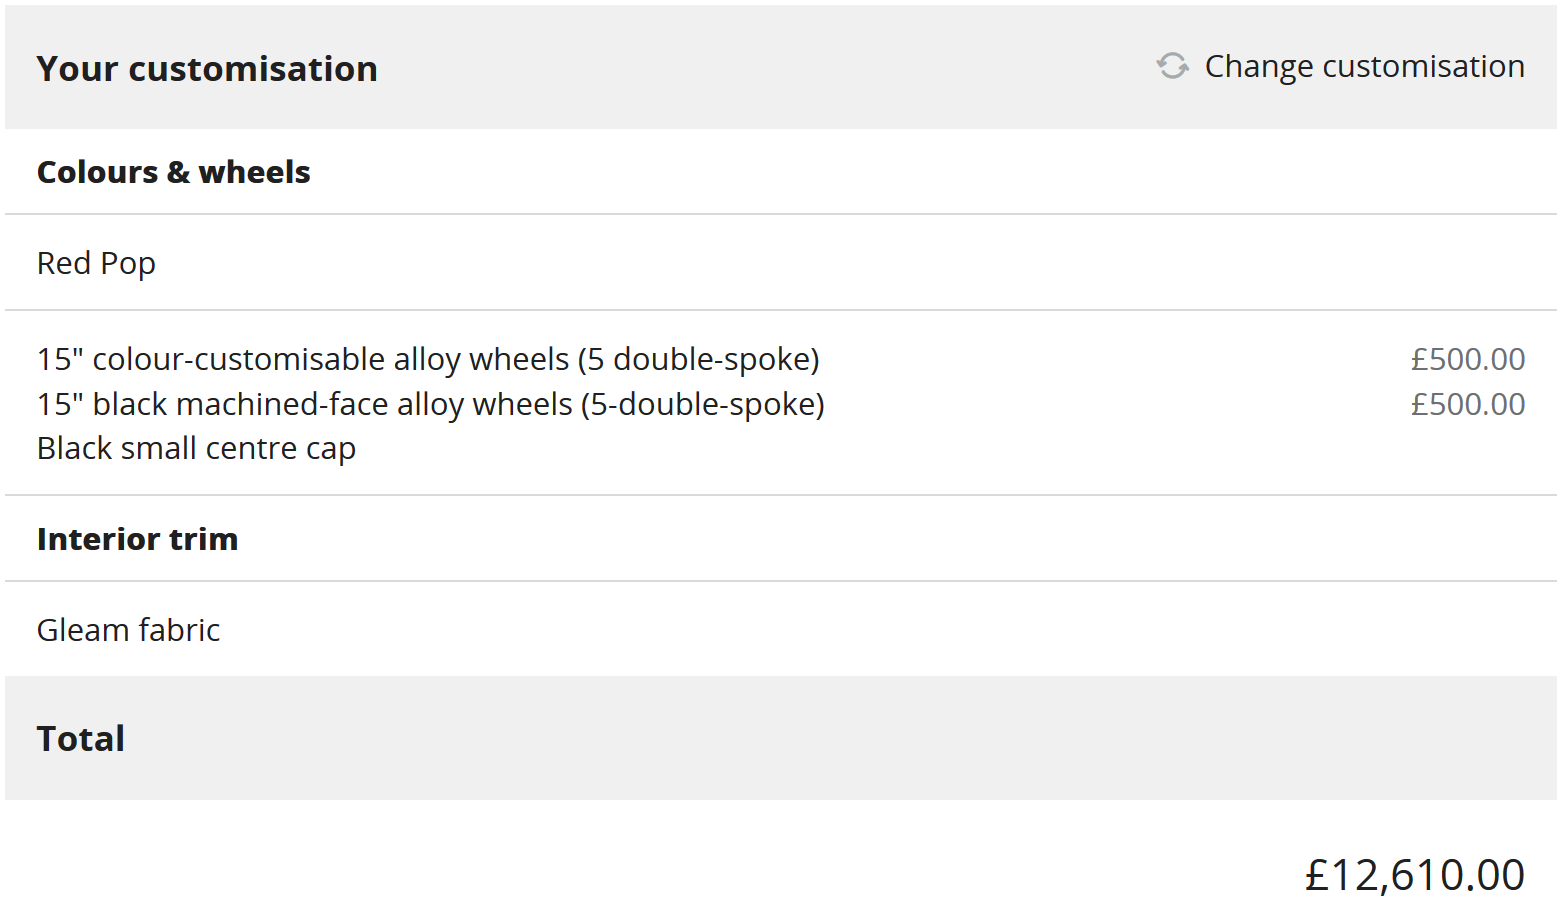
\includegraphics[width=\linewidth]{toyota-aygo-costs3}}}
% \end{frame}

% \begin{frame}{\myframetitle}
% 	\partofpage{70}{\myexampletight{Configuring a German Car}{\includegraphics[width=\linewidth]{bmw-series1-confassistant-blacktooth}}}
% \end{frame}

\subsection{Configurations}

\newcommand{\feat}[1]{{\emph{#1}}}

\begin{frame}{\myframetitle}
	\begin{mycolumns}
		\mydefinition{Configuration}{
			\begin{itemize}
				\item a \emph{configuration} \deutsch{Konfiguration} over a set of features $F$ selects and deselects features in $F$
				\item formally: a pair $(S, D)$ such that $S, D \subseteq F$ and $S, D$ are disjoint ($S \cap D = \varnothing$)
				\item is \emph{complete} \deutsch{vollständig} if all features are covered ($S \cup D = F$) and \emph{partial} \deutsch{partiell} otherwise
				\item a complete configuration is \emph{valid} \deutsch{gültig} if it ``makes sense'' in the domain and \emph{invalid} \deutsch{ungültig} otherwise
				\item we often abbreviate complete configurations with $S \equiv (S, F \setminus S)$
			\end{itemize}
		}
	\mynextcolumn
		\myexample{}{
			Feature set $F = \{ConfigDB, Get, Put, Delete,$
			\hspace*{22mm}$Transactions, Windows, Linux\}$
			
			Examples for \emph{complete} configurations:
			\begin{itemize}
				\item \emph{valid} (read-only database on Windows):
					$\cfg{C, G, W}{P, D, T, L}$
				\item \emph{valid} (fully functional database on Linux):
					$\cfg{C, G, P, D, T, L}{W}$
				\item \emph{invalid} ($\lightning$ no operating system):
					$\cfg{C, G}{P, D, T, W, L}$
				\item \emph{invalid} (transactions $\lightning$ read-only database):
					$\cfg{C, G, T, L}{P, D, W}$
			\end{itemize}
			Examples for \emph{partial} configurations:
			
			$\cfg{C, G}{P, D}$, $(\varnothing, \varnothing)$
		}
	\end{mycolumns}
\end{frame}

\subsection{Characterizing Valid Configurations}

\begin{frame}{\myframetitle}\label{frame:natlang}
	\begin{mycolumns}
		\mynote{Valid Configuration}{
			A complete configuration over $F$ is valid if it ``makes sense'' in the domain.
			\emph{\color{red}{$\leadsto$ ``makes sense''?}}
		}

		\mydefinition{Natural Language}{
			\begin{itemize}
				\item informal description of relationships between features in $F$
				\item a complete configuration $S$ is \emph{valid} if it conforms to the description
				\item[+] succinct
				\item[--] sometimes ambiguous
				\item[--] not machine-readable
			\end{itemize}
		}
	\mynextcolumn
		\myexample{}{
			``A \feat{configurable database} has an API that allows for at least one of the request types \feat{Get}, \feat{Put}, or \feat{Delete}.
			Optionally, the database can support \feat{transactions}, provided that the API allows for Put or Delete requests.
			Also, the database targets a supported operating system, which is either \feat{Windows} or \feat{Linux}.''
		}
	\end{mycolumns}
\end{frame}

\begin{frame}{\myframetitle}\label{frame:cfgmap}
	\begin{mycolumns}
		\mynote{Valid Configuration}{
			A complete configuration over $F$ is valid if it ``makes sense'' in the domain.
			\emph{\color{red}{$\leadsto$ ``makes sense''?}}
		}

		\mydefinition{Configuration Map}{
			\begin{itemize}
				\item a \emph{configuration map} over $F$ is a set of complete configurations $C \subseteq F$
				\item a complete configuration $S$ is \emph{valid} if it occurs in the configuration map ($S \in C$)
				\item also known as product map
				\item[+] precise
				\item[--] not human-readable
				\item[--] redundant, explodes in size ($0 \leq \abs{C} \leq 2^{\abs{F}}$)
			\end{itemize}
		}
	\mynextcolumn
		\myexample{}{
			Feature set $F = \{ConfigDB, Get, Put, Delete,$
			\hspace*{22mm}$Transactions, Windows, Linux\}$
			
			Configuration map:
			
			\small
			\leftandright{
				{\color{black}$\{C,G,W\}$}\\
				$\{C,P,W\}$\\
				$\{C,G,P,W\}$\\
				$\{C,D,W\}$\\
				$\{C,G,D,W\}$\\
				$\{C,P,D,W\}$\\
				$\{C,G,P,D,W\}$\\
				$\{C,P,T,W\}$\\
				$\{C,G,P,T,W\}$\\
				$\{C,D,T,W\}$\\
				$\{C,G,D,T,W\}$\\
				$\{C,P,D,T,W\}$\\
				$\{C,G,P,D,T,W\}$
			}{
				$\{C,G,L\}$\\
				$\{C,P,L\}$\\
				$\{C,G,P,L\}$\\
				$\{C,D,L\}$\\
				$\{C,G,D,L\}$\\
				$\{C,P,D,L\}$\\
				$\{C,G,P,D,L\}$\\
				$\{C,P,T,L\}$\\
				$\{C,G,P,T,L\}$\\
				$\{C,D,T,L\}$\\
				$\{C,G,D,T,L\}$\\
				$\{C,P,D,T,L\}$\\
				{\color{black}$\{C,G,P,D,T,L\}$}
			}
		}
	\end{mycolumns}
\end{frame}

\begin{frame}{\myframetitle}
	\centering
	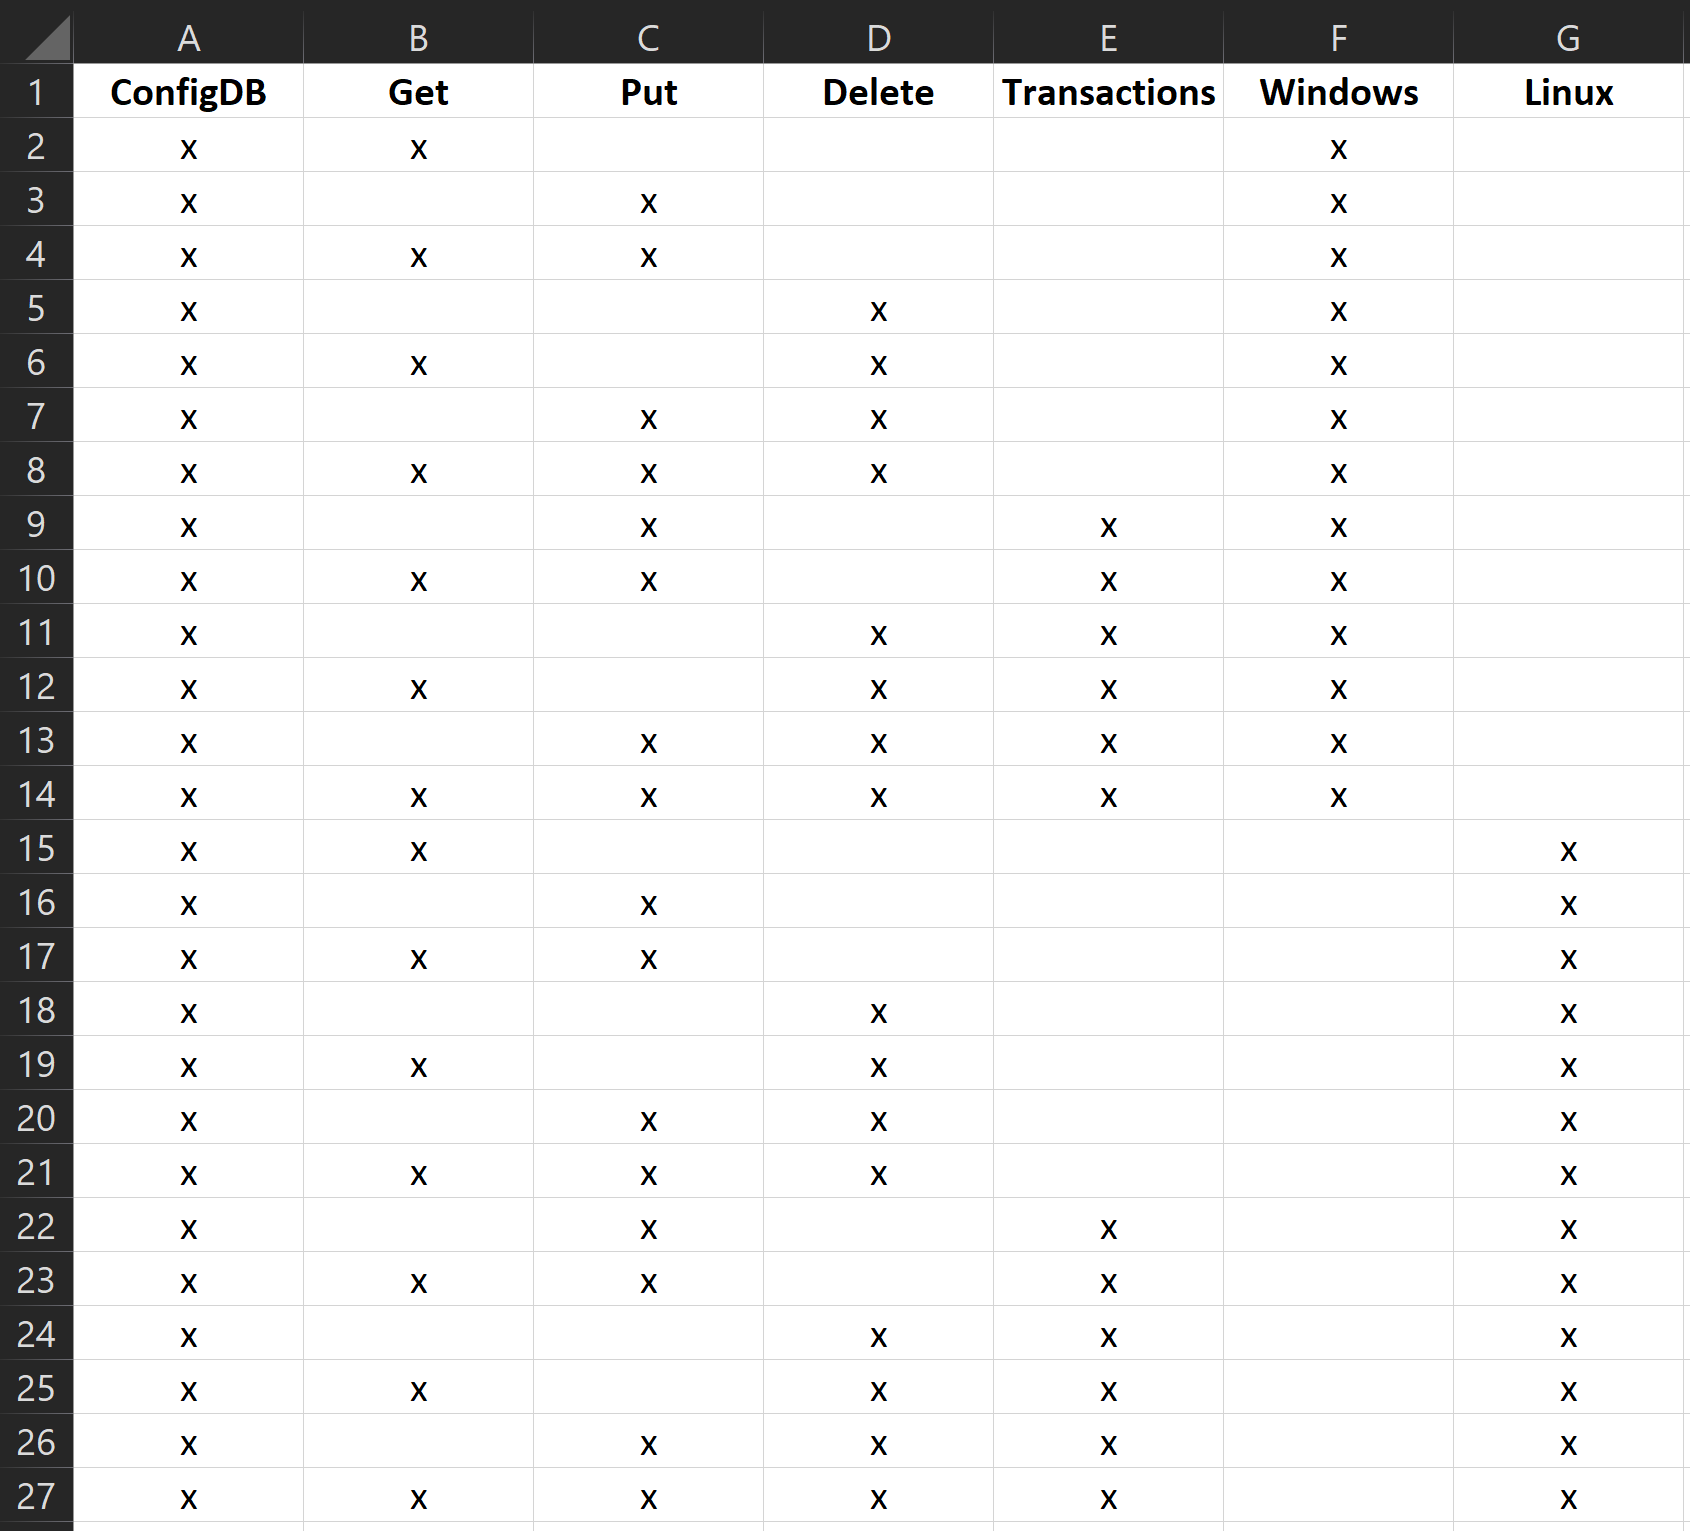
\includegraphics[width=0.48\linewidth]{products-in-excel}

	\textbf{Can we do better?}
\end{frame}

\subsection{Feature Models}

\subsubsection{Syntax}

\begin{frame}{\myframetitle\ \mytitlesource{\fospl}} % \foda?
	\begin{mycolumns}
		\myexampletight{}{
			\centering
			\featureDiagramConfigurableDatabase
			
			\featureDiagramLegend
		}
	\mynextcolumn
		\mydefinition{Feature Model \deutsch{Feature-Modell}}{
			\begin{itemize}
				\item hierarchy of features
				\item dependencies between features modeled by tree and cross-tree constraints
				\item \emph{tree constraints}: defined by the hierarchy
				\item \emph{cross-tree constraints}: propositional formulas over features
				\item \emph{abstract features} are used to group other features
				\item \emph{concrete features} have an implementation
				\item also known as feature diagram or feature tree
    			\item notation for \emph{optional/mandatory features} and \emph{or/alternative groups}
			\end{itemize}
		}
	\end{mycolumns}
\end{frame}

\subsubsection{Semantics}

\begin{frame}{\myframetitle\ \mytitlesource{\fospl}}
	\begin{mycolumns}[animation=none]
		\uncover<2-|handout:1>{
			\mydefinition{Tree Constraints}{
				\begin{itemize}
					\item the \emph{root feature} is always required
					\item each feature requires its parent
					\item an \emph{optional feature} can be (de-)selected freely when its parent is selected
					\item a \emph{mandatory feature} is required by its parent
					\item \emph{or group}: at least one feature must be selected when the parent is selected
					\item \emph{alternative group}: exactly one feature must be selected when the parent is selected
				\end{itemize}
			}
		}
	\mynextcolumn
		\myexampletight{}{
			\centering
			\featureDiagramConfigurableDatabase
		}
		\uncover<3|handout:1>{
			\mydefinition{Cross-Tree Constraints}{
				\begin{itemize}
					\item a list of \emph{propositional formulas} expressing further dependencies between features
					\item each cross-tree constraint must be satisfied
				\end{itemize}
			}
		}
	\end{mycolumns}
\end{frame}

\subsubsection{Example}

\begin{frame}{\myframetitle\ \mytitlesource{\fospl}}
	\begin{mycolumns}[animation=none]
		\myexampletight{}{
			\centering
			\featureDiagramConfigurableDatabase[_fm]
			\featureDiagramOverlay{
				\only<2|handout:0>{
					\featureSelected{(ConfigDB_fm),(API_fm),(Get_fm),(OS_fm),(Windows_fm)}
					\featureDeselected{(Put_fm)(Delete_fm),(Transactions_fm),(Linux_fm)}
				}
				\only<3|handout:0>{
					\featureSelected{(ConfigDB_fm),(API_fm)(Transactions_fm)(OS_fm),(Get_fm)(Put_fm)(Delete_fm),(Linux_fm)}
					\featureDeselected{(Windows_fm)}
				}
				\only<4|handout:0>{
					\featureSelected{(ConfigDB_fm),(API_fm),(Get_fm)}
					\featureDeselected{(Put_fm)(Delete_fm)(Windows_fm)(Linux_fm),(Transactions_fm)(OS_fm)}
				}
				\only<5|handout:0>{
					\featureSelected{(ConfigDB_fm),(API_fm)(Transactions_fm)(OS_fm),(Get_fm),(Linux_fm)}
					\featureDeselected{(Put_fm)(Delete_fm)(Windows_fm)}
				}
			}
		}
	\mynextcolumn
		\myexample{Is This a Valid Configuration?}{
			\begin{itemize}
				\item<2-|handout:1> \emph{valid} (read-only database on Windows):
					$\cfg[2|handout:0]{C, A, G, O, W}{P, D, T, L}$
				\item<3-|handout:1> \emph{valid} (fully functional database on Linux):
					$\cfg[3|handout:0]{C, A, G, P, D, T, O, L}{W}$
				\item<4-|handout:1> \emph{invalid} ($\lightning$ no operating system):
					$\cfg[4|handout:0]{C, A, G}{P, D, T, O, W, L}$
				\item<5-|handout:1> \emph{invalid} (transactions $\lightning$ read-only database):
					$\cfg[5|handout:0]{C, A, G, T, O, L}{P, D, W}$
			\end{itemize}
		}
	\end{mycolumns}
\end{frame}

\begin{frame}{\myframetitle}
	\begin{mycolumns}
		\todo{graph product line example from Timo}

		%\centering
		%\featureDiagramWaffle
	\mynextcolumn
		\mynote{Notation}{
			\begin{itemize}
				\item abstract and concrete features can be assigned arbitrarily
				\item groups can be used anywhere
				\item directly below groups, no optional or mandatory markers are allowed
			\end{itemize}
		}
	\end{mycolumns}
\end{frame}

\subsection{Advantages of Feature Modeling}
\begin{frame}{\myframetitle}
	\begin{mycolumns}
		\textbf{Making Tacit Knowledge Explicit}
		\mynote{Interview with Practitioners \mysource{\href{https://link.springer.com/chapter/10.1007/978-3-319-11653-2_19}{Berger~et~al.~2014}}}{
			\mycite{I think the best [about feature modeling] is you can see relationships, to actually know what configurations are allowed and what are not allowed. That was also not so easy to express in the past [\ldots] This is from the developer's point of view. But it's also, we can see that from the, say project development, it's also important, because before we noticed that \emph{the same functionality was implemented twice} within the same project, basically they haven't realized that. They implemented the same features.}
		}
	\mynextcolumn
		\textbf{Tool Support}

		\pic[width=\linewidth]{featureide-feature-model-editor}
	\end{mycolumns}
\end{frame}